\begin{itemize}
    \item Traditional algorithms: estimating the expected reward and epistemic uncertainty. 
    \item In real-world scenarios, distributional features such as multimodality, skewness, and heavy tails, reflecting aleatoric uncertainty, can provide valuable information for decision-making.
\end{itemize}
    \begin{minipage}[t]{0.45\linewidth}
    \vspace{10pt} % 强制顶部对齐
    This project investigates a method that makes decisions by directly sampling from the full conditional reward distribution $P(r \mid c, a)$, which is learned through a diffusion model.
    \end{minipage}
\hfill
\begin{minipage}[t]{0.48\linewidth}
\vspace{0pt}
    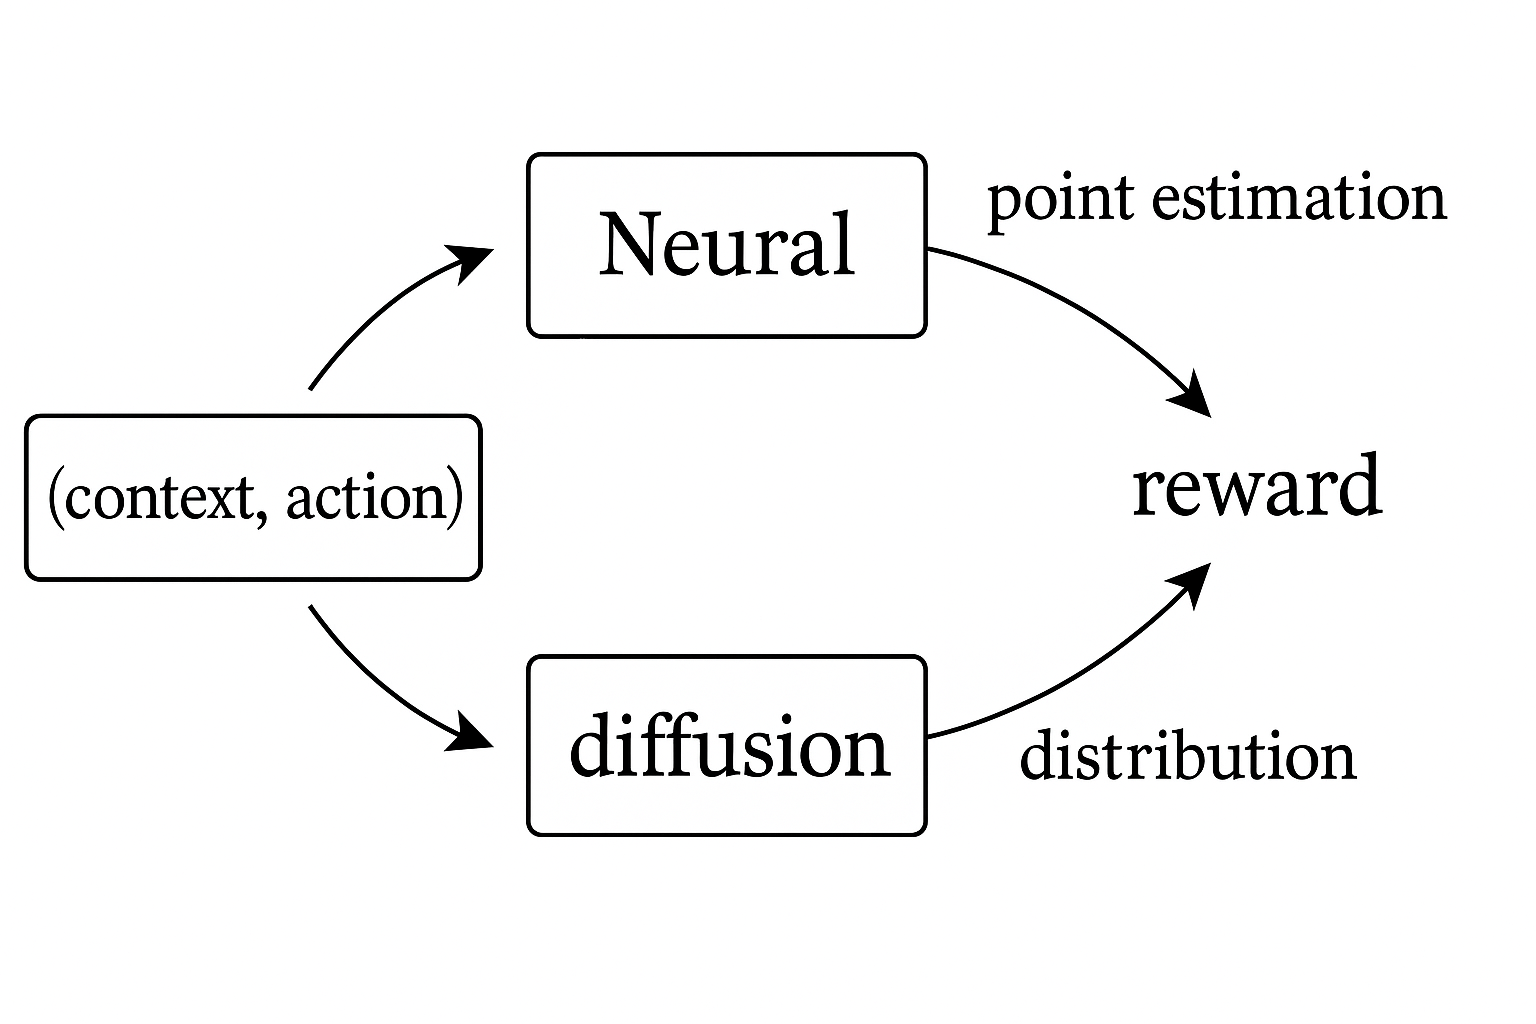
\includegraphics[width=\linewidth]{Img/context_diffusion.png}
\end{minipage}
\textbf{Reward Distribution Modeling:}

Pretrain: A diffusion model is trained on $(c, a, r)$ data to approximate $P(r \mid c, a)$.

\textbf{Action Selection (at context $c_t$):}
\begin{enumerate}
    \item For each action $a$: sample $\tilde{r}_a \sim P(r \mid c_t, a; W_{\text{diffusion}})$ using the trained diffusion model.
    \item Choose action: $a_t = \arg\max\limits_{a \in \mathcal{A}} \tilde{r}_a$.
\end{enumerate}